\documentclass{book}
\usepackage{mathtools}
\usepackage{tikz}
\usetikzlibrary{positioning}

\usepackage{amsthm}
\usepackage{amsmath}
\usepackage{amssymb}

\newtheorem{defn}[equation]{Definition}
\newtheorem{coro}[equation]{Corollary}
\newtheorem{prop}[equation]{Proposition}
\renewenvironment{proof}{\emph{Proof}}{\qed}


\begin{document}






\tableofcontents

\emph{I'd like to include a table here with mathematical notation, giving brief explanations for what symbols such as $\in$, $\subset$, $\mathbb{R}$, etc. mean, just in case the reader isn't familiar with them.}

\clearpage






\section{Foreword}
In transitioning to advanced classes, a physics student will find their familiar mathematical tools are inadequate to describe certain physical phenomena. The methods of traditional vector calculus in three dimensions, though very useful in electromagnetism and classical mechanics, are not always usable in higher dimensions, such as those used in general relativity and Hamiltonian mechanics. For that, we need differential geometry. When trying to learn a subject in mathematics, however, you tend to find books written for mathematicians, in a language that mathematicians are familiar with. As such, they are filled with long, obtuse definitions and prose that, while mathematically very precise, isn't exactly light reading, and can even be overkill for a proper physical understanding. 

What follows is a purely physical treatment of differential geometry used in physics. While it is less mathematically rigorous than a typical textbook, the hope is that the reader will be able to gain a geometric intuition for the math they use, so that the math isn't simply a black box beyond understanding, and that further study in the subject will be aided by a solid grounding here. The focus is always on readability, applicability, and physicality, so pictures are prevalent throughout. 

We assume on the part of the reader a class in introductory classical mechanics and electromagnetism, as well as vector calculus. More advanced topics in physics and mathematics may be touched on, but only for the use of giving an example, or demonstrating the usefulness of these mathematical tools. 


\chapter{Mathematical representations of physical objects}



\section{Physical objects and quantities}

At the heart of scientific investigation is the identifying and organizing of objects based on their properties, through measurement and experiment. This could be anything from setting a block on a scale to determine its weight to determining the species that a particular animal belongs to. For our purposes here, we will be dealing only with properties that can be described using real numbers, such as mass, temperature, velocity, etc. The identification of a particular physical property with a real number is a \textbf{quantity}.

\begin{defn}
	A \textbf{quantity} is a function $q : U \to \mathbb{R}$ that assigns a measurable value to a physical case.
\end{defn}



It's possible, however, that we won't be able to distinguish between two objects with only one quantity. Say, for instance, that we're talking about weather. Knowing what the temperature will be tomorrow is certainly useful, but as anyone from Florida can tell you, 80$^o$F with 95$\%$ humidity is very different from 80$^o$F with 30$\%$ humidity. In distinguishing objects, then, we will often want to define more than one quantity. By defining enough quantities to distinguish one object from another, but not so many such that we have redundancies, we can define a \textbf{coordinate system}.


Normally, we think of coordinate systems in the context of quantifying an object's position, in terms of its x-, y-, and z-coordinates. Though it may be an abuse of terminology, we will use the same phrase to describe coordinates in other contexts. Consider, for instance, phase space. Configurations in phase space are fully characterized by position and momentum, which would be our two quantities, thus giving us a coordinate system. To give another example, we can look at a system described by the ideal gas law. With this, we would create a coordinate system with pressure, volume, and temperature. 

\begin{defn}
	A \textbf{coordinate system} $Q$ is a collection of $n$ quantities $q^i : U \to \mathbb{R}^n$ such that there is a one-to-one relationship between the physical objects in $U$ and elements of $\mathbb{R}^n$.
\end{defn}



With coordinate systems now defined, we recognize that in many instances, two different coordinate systems function just as well to describe a certain object. Mathematically, this occurs when two sets, each with defined coordinate systems, overlap. The points that lie within this overlapping section may be described in either coordinate system. To give an example from geography, consider an atlas of the world: a collection of maps. Depending on the atlas you're looking at, certain places may show up in multiple maps. Consider Moscow, for instance. It could very well show up on a map of Asia, perhaps in a square labeled B2, while also showing up on a map of Europe, perhaps in a square labeled C8. Either way of describing Moscow's position is equally valid, and you can freely "transform" between the coordinate systems as far as Moscow is concerned. Alternatively, consider the "point" Lisbon. Lisbon will show up on a map of Europe, perhaps in square F1, but you would never find Lisbon on a map of Asia. Therefore, its position may only be described in terms of the coordinates on the map of Europe.


\begin{defn}
	Given two coordinate systems  $Q : U \to \mathbb{R}^n$ and $Q' : V \to \mathbb{R}^n$ such that $U \cap V \neq \emptyset$, we call a \textbf{coordinate transformation} the function $f = Q' \circ (Q)^{-1} : \mathbb{R}^n \to \mathbb{R}^n$.
\end{defn}



\textbf{May have to describe the meaning of the diagram, reader might not know. Could be talked about with the notation table in the beginning}

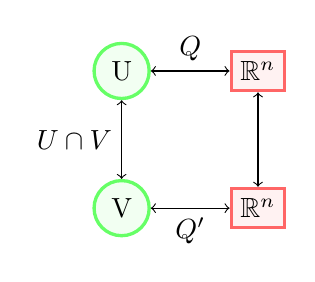
\begin{tikzpicture}
[roundnode/.style={circle, draw=green!60, fill=green!5, very thick, minimum size=7mm},
squarednode/.style={rectangle, draw=red!60, fill=red!5, very thick, minimum size=5mm},
]
\node[roundnode]	(U) {U};
\node[roundnode]	(V) [below=of U]{V};
\node[squarednode]	(realU) [right=of U] {$\mathbb{R}^n$};
\node[squarednode]	(realV) [right=of V] {$\mathbb{R}^n$};

\draw[<->] (U) -- (realU) node[midway, above] {$Q$};
\draw[<->] (U) -- (V) node[midway, left] {$U\cap V$};
\draw[<->] (V) -- (realV) node[midway, below] {$Q'$};
\draw[<->] (realU) -- (realV);
\end{tikzpicture}


Because of the poles, every location on Earth cannot be equally quantified with only one set of coordinates. This can be plainly seen on a typical flat map, such as a Mercator Projection. Land proportions grow the closer to a pole they are, making Greenland appear massive, and the Sahara proportionally far smaller. Furthermore, because the poles have in a sense been unraveled, the South Pole, which ought to be a single point, is an entire line along the southern edge of the map. A proportionally accurate projection of the Earth onto a flat surface requires at least two separate maps. For instance, you could have a map of the top hemisphere, centered at the north pole, and then of the bottom hemisphere, centered at the south pole. The Earth then motivates the introduction of \textbf{manifolds}. 


\textbf{Insert a picture of the Mercator Projection}

\textbf{Insert pictures of "polar" projections}

\begin{defn}
	A \textbf{manifold} is a set of physical objects $X$ such that for any $x \in X$ there exists a $U \subset X$ that contains $x$ and upon which a coordinate system $Q$ is defined. Manifolds have dimensionality, as determined by the dimension of their coordinate systems.
\end{defn}


Earlier, weather was given as an example of a set of possible cases of a system, with readings such as temperature and humidity allowing us to define a coordinate system. In this context, the "manifold" would be the set of possible weather configurations, with each point being a single weather report. Another example of a manifold would be the possible results of a blood drawing. The doctor takes your blood for analysis, the results of which are collected on a report, detailing things such as blood pressure, cholesterol levels, white blood cell count, etc. Further examples include: 

\begin{itemize}
\item The conditions of your car, with the dials on the dashboard being your method of reading them 

\item The freight on a ship, with the bill of lading detailing amounts

\item Any sort of information that can be condensed down to a series of real numbers

\end{itemize}

The variety of examples is to show the ubiquitousness of manifolds, and that they are very familiar, everyday objects. This versatility proves their usefulness in physics, and in scientific investigation in general. But unlike in the case of the Earth, manifolds do not in general come prepackaged with a notion of distance. What does it mean, for instance, for there to be distance between weather reports? Perhaps you can argue that distance comes into play by specifying where exactly the weather report was taken, but this is simply the geography example again under a different name. No, in order to define distance on our manifolds, we will need to wait until Chapter 3. 


\section{Sub-manifolds and k-surfaces}

Consider again the weather report example, where we are taking into account where exactly the report was taken. Perhaps we decide that we no longer care about what the actual weather reading is, instead worrying only about where we are. This takes us immediately from one example of a manifold to another, where the latter has fewer dimensions than the former, and where any point on the latter is also a point on the former. Thus, geography is a \textbf{submanifold} of the weather report.


\begin{defn}
	Consider a manifold X of dimension n, and a manifold Y of dimension k, such that $k \leq n$. Y is a \textbf{submanifold} or a \textbf{k-surface}\footnote{In general, we will be using the term "k-surface", instead of "submanifold." There will be many terms throughout this thesis prefaced by "k-". In general, this means that the object in question has k dimensions, and can be organized by their dimensionality.} of X if any point on Y is also a point on X. 
\end{defn}

\begin{tikzpicture}
[roundnode/.style={circle, draw=green!60, fill=green!5, very thick, minimum size=7mm},
squarednode/.style={rectangle, draw=red!60, fill=red!5, very thick, minimum size=5mm},
]
\node[roundnode]	(X) {X};
\node[roundnode]	(Y) [below=of X]{Y};
\node[squarednode]	(realX) [right=of X] {$\mathbb{R}^n$};
\node[squarednode]	(realY) [right=of Y] {$\mathbb{R}^k$};

\draw[<->] (X) -- (realX) node[midway, above] {$Q$};
\draw[->] (X) -- (Y) node[midway, left] {$U\cap V$};
\draw[<->] (Y) -- (realY) node[midway, below] {$P$};
\draw[->] (realU) -- (realV);
\end{tikzpicture}



\begin{defn}
	For some manifold X of dimension n, $S^k$ is the set of all possible \textbf{k-surfaces} of dimension $k \leq n$, and S $=$ $\cup^n_{k=0}S^k$ is the set of all surfaces. 
\end{defn}

We can go even further in our description of k-surfaces. If we assume that we can freely move through the entirety of the Earth's crust, but may not leave the surface of the Earth, we may say that the Earth manifold has a \textbf{boundary}, that being the surface of the Earth. Because radius is held fixed on the surface, the boundary of the Earth has a dimensionality of 2, instead of 3. 

\begin{defn}
	Given k-surface $\sigma^k \in S^k$, the \textbf{boundary} of $\sigma^k$, denoted by $\partial\sigma^k \in S^{k-1}$ is the limit of varied coordinates. Points lying on the boundary are called \textbf{boundary points.}
\end{defn}


If instead of holding one value fixed and allowing the others to vary, and thereby forming a boundary, we could choose instead to allow one quantity to vary and hold the others fixed. For instance, say in the example of the weather report, we wish to vary only temperature. On the manifold containing all weather reports, this varying of only temperature would manifest itself as a line on the manifold, the points on which being weather reports whose values for all quantities besides temperature are identical. 

\begin{defn}
	A \textbf{coordinate line} is the set of points in $\mathbb{R}^n$ obtained by allowing one quantity to vary and holding the others fixed. 
\end{defn}

\begin{defn}
	A \textbf{coordinate k-surface} is the set of points in $\mathbb{R}^n$ obtained by allowing k quantities to vary and holding (n-k) quantities fixed.  
\end{defn}


Now that we have k-surfaces, we have a notion of where points lie relative to some k-surface. When varying coordinates to creates coordinate lines, surfaces, volumes, etc., the varying can be brought to a halt by the geometry of the object that we're working on. Where the varying ends lies the boundary of our surface. 





Intuitively, we can talk about the boundary of a k-surface being a wall, beyond which a point confined to the k-surface cannot go. Consider, for instance, a particle confined to the inside of a sphere. The particle is free to move anywhere within the sphere, but is stopped from leaving by the surface of the sphere itself. Thus, the surface is the boundary. On the other hand, consider a particle confined to the surface of a sphere. The particle can travel along the surface as long as it wants without being stopped by any kind of wall. Thus, the surface of a sphere does not have a boundary. \textbf{Probably have a picture}

We can map between a k-surface and its boundary, if it exists, with the \textbf{boundary operator}. I.e., if $\sigma^2$ is a sphere, $\partial \sigma^2$ is its boundary: its surface. It follows also from the argument in the proceeding paragraph that $\partial\partial\sigma^2$ is empty. This is offered without formal proof, but is true for general k-surfaces. 

\begin{defn}
	For k-surface $\sigma^k \in S^k$, the \textbf{boundary operator} $\partial : S^k \to S^{k-1}$ gives the set of boundary points of $\sigma^k$. 
\end{defn}

\begin{coro}
	Given $\sigma^k \in S^k$, $\partial \sigma^k \in S^{k-1}$, and $\partial\partial \sigma^k = \emptyset$. 
\end{coro}


\section{Linear Functionals of K-surfaces}
\textbf{Conservative force is exterior derivative of some potential, and is therefore closed (ext derivative is 0) and exact. A nonconservative force will not be closed, but can be discussed using one-forms}

\textbf{Path independence is not necessary to talk about. The functional depends on the path. If it only depends on the beginning and end points, it's a boundary functional. Say "Force dpeends on the path and that's good. Later the force only depends on the starting and end, then it's a boundary functional / gradiant of some scalar field"}

Say we have a path on our manifold (that is, a 1-surface), along which we want a particle to travel, and suppose we have a force in play with some sort of effect on the particle. We can define a work function $W$ which, with the aforementioned defined force, takes a path $\lambda$ and returns the work (a scalar) necessary to move the particle along that path. More concretely, say we have a line $\lambda$ with starting point $a$, ending point $c$, and some middle point $b$. We can say that 
\begin{gather} W(\lambda_{a \to c}) = W(\lambda_{a \to b}) + W(\lambda_{b \to c}).
\end{gather}
 The work function is thus a linear function along a 1-surface: a \textbf{1-functional}. Furthermore, just as 1-surfaces are a specific subset of k-surfaces, we can say that 1-functionals are a specific subset of \textbf{k-functionals}, which in general will be functions along k-surfaces. 




\begin{defn}
	A \textbf{linear function of k-surfaces}, or \textbf{k-functional}, is a function $f_k : S^k \to \mathbb{R}$ such that:
	
	I. $f_k$ is linear: for $\sigma^k_1$, $\sigma^k_2 \in S^k$, if \begin{gather}\sigma^k_1 \cap \sigma^k_2 \subseteq \partial \sigma^k_1 \cup \partial \sigma^k_2\end{gather}, then \begin{gather}f_k(\sigma^k_1\cup \sigma^k_2) = f_k(\sigma^k_1) + f_k(\sigma^k_2) \end{gather};
	
	II. $f_k$ commutes with the limit. That is, the limit of the function is the function of the limit. 
\end{defn}

\textbf{Still not a clear explanation}
The second point in this definition must be remarked on, and it will be clarified with an example: the length of a line is not a k-functional. The length of a line $\lambda$ is equal to the sum of the magnitudes in the length's constituent directions. So, for a line $\lambda \in \mathbb{R}^2$ with components x and y, the length $L = \sqrt{x^2 + y^2}$. This is \emph{not} the same as the sum of the individual lengths, which would be just $x + y$. Simply put, the length of the limit is not the same thing as the limit of the length. 


\begin{defn}
	$F_k$ is the set of all functionals of dimension k, and $F = \cup_{k=0}^nF_k$ is the set of all functionals. 
\end{defn}


In the most general case, the work done along a path will depend on the path itself. For certain forces, however, the work done will depend only on the starting and ending points of the path. That is, it depends only on the \emph{boundary} of the path. This implies that for such a force, if the path is closed (i.e., the starting and ending points are the same), the total work done will be zero. Forces that do path-independent work are called conservative, while those that do not are called nonconservative. 

The boundary of a k-surface is a (k-1)-surface, which can be passed to a (k-1)-functional. Just as we can relate a k-surface to its boundary, we can relate a k-functional to the (k-1)-functional. In complement to the boundary operator $\partial$, we define the \textbf{boundary functional} $\eth$. 



\begin{defn}
	$\eth : F_k \to F_{k+1}$ such that $\eth f_k(\sigma^{k+1}) = f_k(\partial \sigma^{k+1})$ is the \textbf{boundary functional} on k-functionals. 
\end{defn}

\begin{prop}
	Let $f_k \in F_k$ be a k-functional, then $\eth\eth f_k = 0 $.
	
\end{prop}
\begin{proof}\\
	This property follows easily from the relation in Definition 1.14.\\ 
	Let $f_k : S^k \to \mathbb{R}$, $g_{k+1} : S^{k+1} \to \mathbb{R},$ and $h_{k+2}: S^{k+2} \to \mathbb{R}$ be linear functions, and let $\sigma^k$ be an element of $S^k$. \begin{gather}f_k(\sigma^k) = g_{k+1}(\partial \sigma^k) = h_{k+2}(\partial\partial \sigma^k) = f_k(\emptyset) = 0.\end{gather} 
	
	So, $h^{k+2}(s) = 0$ $\forall$ $\sigma^k$, and $h^{k+2}$ is the zero function. 
\end{proof}\\

If we have a work function and pass it a path with length zero, the function will return, of course, zero. It is true in general, and offered without formal proof, that a k-functional given an empty set will return zero. 

\begin{prop}
	A k-functional applied to the empty set gives zero. 
\end{prop}





\section{Summary}


In this first section, we've laid the groundwork for a physical treatment of differential geometry. By starting with the idea of distinguishing objects through quantities, we are quickly able to come to an intuitive understanding of manifolds. We see also that a purely physically motivated form of differential geometry is possible, which will be further confirmed in the coming chapters. 


\chapter{Mathematical representation of infinitesimal objects}


\section{Differentiable manifolds}

In the previous section, we began to discuss functionals applied over k-surfaces. With the rules we've established, we can break up a k-surface into multiple sections, such that applying a functional over the entire surface is equivalent to applying it to each of the sections individually, and then summing their contributions. What if we could make these sections infinitesimally small? How would our manifolds behave, and furthermore, what happens to the functionals?

Consider now a k-surface $\sigma^k \in S^k$, with a k-functional $f_k$. We can break this surface up into "n" number of parts, called $\sigma^k_1, \sigma^k_2, ..., \sigma^k_n$. We know that \begin{gather} f_k(\sigma^k) = f_k(\sigma^k_1) + f_k(\sigma^k_2) + ... + f_k(\sigma^k_n) = \Sigma^n_if_k(\sigma^k_i).\end{gather} If we let n tend to infinity, the parts become infinitesimal. Summing the contributions of the infinitesimals is equivalent to an integral of the function over the whole surface. So, for k-surface $\sigma^k \in S^k$ and k-functional $f_k: S^k \to \mathbb{R}$, $f_k(\sigma^k) = \int_{\sigma^k}\omega_k(d\sigma^k)$ for some yet undefined function $\omega_k$. The existence of infinitesimals on our manifolds allows us to perform calculus. Such manifolds are \textbf{differentiable manifolds}. 

Technically speaking, differentiability is a property not of the manifold, but of the coordinate systems that are defined on it. And furthermore, not every coordinate system is differentiable. In order to maintain differentiability on our manifolds, we will be constraining ourselves to coordinate systems which are differentiable. Essentially, what we're doing here is looking at an entire manifold, with all of its constituent subsections and thereon defined coordinate systems, and disregarding the coordinate systems that are not differentiable. This property manifests itself as the coordinate transformation between subsets of the manifold being smooth. 


\begin{defn}
	A \textbf{differentiable manifold} is a manifold $X$ of dimension $n$ such that if there are overlapping subsets $U$ and $V$ with defined coordinate systems $Q: U \to \mathbb{R}^n$ and $Q': V \to \mathbb{R}^n$, then the coordinate transformation $f = Q \circ Q'^{-1}$ is smooth. 
\end{defn}





\section{Vectors and Covectors}


This section and the next will be focusing on the formalism of functions over infinitesimals. Here we will be starting with the k = 1 case, and seeing what mathematical tools naturally arise. In the next section, we will be moving to the general k case, and seeing how the math here in turn generalizes. 


Let $W \in F_1$ be the work function with a force as described in section 1.3, and let $\lambda \in S^1$ be the line that we are passing it. So, we can say that $W(\lambda) = \Sigma^n_iW(\lambda_i)$, where the ending point of each $\lambda_i$ is the starting point of each $\lambda_{i+1}$. Letting n tend to infinity, this expression becomes $W(\lambda) = \int_{\lambda} f(d\lambda)$ for a force $f$. Each $d\lambda$ represents an infinitesimal segment along the line $\lambda$ which, if summed together, will return $\lambda$. We call the infinitesimal segments of our line \textbf{vectors}. 

As we are breaking up the line into infinitesimal segments, we see that the functional applied over the line takes an infinitesimal form as well. The work function has become a force that takes a vector and returns that vector's contribution to the overall work. Such functions applied over infinitesimals are called \textbf{covectors}. 


Concretely, consider a spring with spring constant $k$ and with a mass $m$ attached to the end, oscillating without drag. The work necessary to pull the mass from the point $x = a$ to $x = b$ (being the starting and ending points of the line $\lambda$) is $W(\lambda) = \int_a^b -kx dx$.\footnote{We are technically getting ahead of ourselves here by presenting the function with specific coordinates. We have been entirely coordinate-free so far, and will have to wait until section 2.4 for the discussion of working with coordinates} The force (the covector) is $-kx$, and the infinitesimal segment (the vector) is $dx$. In general, a 1-functional over a 1-surface is the integrated form of a covector over vectors.


\begin{defn}
	A \textbf{vector} $v^1 \in V^1$ is an infinitesimal segment along a line. A \textbf{tangent space}, then, is a collection of vectors that share a fixed point. 
\end{defn}


\begin{defn}
	A \textbf{covector} $\omega_1 : V^1 \to \mathbb{R}$ is a linear function of vectors. 
\end{defn}


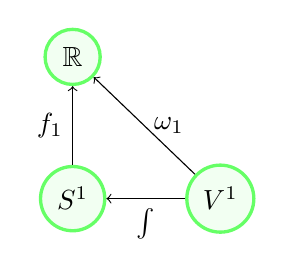
\begin{tikzpicture}
[roundnode/.style={circle, draw=green!60, fill=green!5, very thick, minimum size=7mm},
squarednode/.style={rectangle, draw=red!60, fill=red!5, very thick, minimum size=5mm},
]
\node[roundnode]	(r) {$\mathbb{R}$};
\node[roundnode]	(s) [below=of r]{$S^1$};
\node[roundnode]	(v) [right=of s] {$V^1$};

\draw[->] (v) -- (s) node[midway, below] {$\int$};
\draw[<-] (r) -- (v) node[midway, right] {$\omega_1$};
\draw[->] (s) -- (r) node[midway, left] {$f_1$};
\end{tikzpicture}



\begin{prop}
	All linear 1-functionals have a corresponding covector, such that for $f : S \to \mathbb{R}$, $f = \int_{\lambda} \omega_1(d\lambda)$. In words, a linear functional applied over a line is the same as an integral of a covector over the infinitesimal segments of that line. Functionals may only be valid on certain patches in our space, however, meaning that we cannot necessarily define a form that works everywhere. 
\end{prop}




\section{K-vectors and K-forms}

Let $\Phi \in F_2$ be a functional for magnetic flux; that is, the function that gives the "flow" of magnetic field through some surface, and let $\sigma \in S^2$ be such a surface. Mathematically, this is another example of a k-functional being passed a k-surface, and returning a real number. So, we may write that \begin{gather}\Phi(\sigma) = \Phi(\sigma^1) + \Phi(\sigma^2) + \Phi(\sigma^3) + ... = \sum_{i=1}^n \Phi(\sigma^i),\end{gather} which becomes $\int_\sigma B(d\sigma)$ as n tends to infinity. This appears to be identical to the case where k=1. The difference comes in by realizing that the surface $\sigma$ may not be broken up into infinitesimal line elements. Rather, we have to use infinitesimal paralellograms. Just as $\Phi$ is a 2-functional and $\sigma$ a 2-surface, we call the infinitesimal parallelograms d$\sigma$ 2-vectors, and B a 2-form. Incidentally, just as the work 1-functional became force as a covector (in other words, a 1-form), the flux as a 2-functional became the magnetic field as a 2-form. We see that the general relationship between forms and functionals, and vectors and surfaces carries over into the two dimensional case.  


We propose that in the general kth case, we can through integration connect our forms with functionals, and vectors with surfaces. Let $f_k \in F_k$ be a k-functional and $\sigma^k \in S^k$ a k-surface. We can say that \begin{gather}f_k(\sigma^k) = \sum_{i=1}^n f_k(\sigma^k_n) = \int_{\sigma^k} \omega_k(d\sigma^k)\end{gather} as n tends to infinity for some function $\omega_k$. We call $\omega_k$ a \textbf{k-form}, and d$\sigma^k$ a \textbf{k-vector}. 

Using line segments or parallelograms as our infinitesimal elements is not sufficient on a k-surface. At this point, we must make use of infinitesimal \emph{parallelepipeds}: a k-dimensional shape whose sides are (k-1)-parallelepipeds. Whereas before when the line segments would be stuck end-to-end, the parallelepipeds will be stuck side-to-side, such that one side of one parallelepiped makes up one side of the other. We can say that the infinitesimal elements in the cases of k=1 and k=2 are still parallelepipeds. In the case of k = 1, an infinitesimal segment may be thought of as a parallelepiped without width or height. By that same thinking, when k = 2, an infinitesimal area on a 2-surface may be thought of as a parallelepiped without height. 


\begin{defn}
	A \textbf{k-vector} $v^k \in V^k$ is an infinitesimal parallelepiped on a k-surface. A vector as discussed previously is a 1-vector. 
\end{defn}


\begin{defn}
	$V^k$ is the set of all vectors of rank k and $V = \cup_{k=0}^n V^k$ is the set of all vectors. 
	\end{defn}
 

\begin{defn}
	A \textbf{k-form} $\omega_k : V^k \to \mathbb{R}$ is a linear functional that converts an infinitesimal parallelepiped into a scalar value. A covector as discussed previously is a 1-form. 
\end{defn}

A k-form may operate on multiple vectors if the sum of the ranks of the vectors equal k. That is, for $v^i \in V^k$ and $v^j \in V^j$, such that $i + j = k$, we write $\omega_k(v^i, v^j)$ to say that $\omega_k$ has been passed two vectors, from which we will get a single scalar. 


\begin{defn}
	$\Omega_k$ is the set of all forms of dimension k and $\Omega = \cup_{k=0}^n\Omega_k$ is the set of all forms. 
\end{defn}

To finish up the generalization of the previous section, we establish the relationship between k-functionals and k-forms, between k-surfaces and k-vectors. The latter two are infinitesimal variants of the former two, and are related to one another by an integral. 


\begin{prop}
	Every linear k-functional has a corresponding k-form, such that for $f_k : S^k \to \mathbb{R}$, $f_k = \int_{\sigma^k} \omega_k(d\sigma^k)$. In words, a linear functional applied over a k-surface is the same as an integral of a k-form over the infinitesimal parallelepipedes of that k-surface. 
\end{prop}

\textbf{(Look up geometric measure theory. Highlight in the introduction that the definitions as we put them don't give diff forms (because the space isn't specifically differentiable, since we can add discontinuities and still end up with the same integral), but that this gives the right intuition. For a density, add a constant at a particular point. It doesn't change the over all mass. Take a force and increase it by a constant at a particular point, doesn't change the overall work)}

A clarification must be made now. In most treatments of electromagnetism, the magnetic field $B$ is what a pseudeovector. What this means is that $B$ behaves as a vector when undergoing rotation, but when undergoing reflection gains an additional sign flip. This particular characterization of $B$ depends on a notion of perpendicularity that is true for $\mathbb{R}^3$, but isn't for $\mathbb{R}^4$ and above, and is also the reason why we will not be using the cross product in our discussion here. The cross product depends on there being only one linearly independent direction normal to a surface, which is the case in $\mathbb{R}^3$. In $\mathbb{R}^4$ on the other hand, there are \emph{two} directions normal to each surface, and in general n-dimensional space, there will be (n-2) linearly independent perpendiculars. What we do instead is keep track of components using the two directions tangent to the surface, rather than by the direction normal to the surface (i.e., $B^z$ is actually $B^{xy}$). Furthermore, the cross product requires that angles be defined, from which comes perpendicularity and the normal vector, and the reader may have noticed that we have not yet given any notion of angles (that comes in chapter 3). 



Consider the problem now of constructing surfaces, volumes, and their higher dimensional equivalents. Arranging two 1-vectors $\vec{a}$ and $\vec{b}$ such that they both share a starting point allows one to construct a paralellogram (a 2-vector) with sides made up of the 1-vectors. The area and orientation of this 2-vector depends on the magnitudes and orientations of the two component 1-vectors. In 3D space, this orientation would be the line normal to the 2-surface, but we are not necessarily in 3D space. By flipping the direction of one of the vectors, the area of the resulting 2-vector would be the same as before, but the orientation (the normal) would be flipped. What's happening here is that we are combining two 1-vectors to create a 2-vector. This same mechanism works for a 1-vector and a 2-vector, creating a 3-vector, as well as for the arbitrary m-vector and n-vector, creating an (m+n) vector (though for vectors of degree greater than three, this is much harder to visualize). We require also that our method for combining k-vectors is anticommutitive or skew-symmetric; that is, by flipping the order of the components, the magnitude remains the same, but the orientation flips. The tool that does this is the \textbf{wedge product}.
\textbf{Probably put a picture of that here}



\begin{defn}
	
	The \textbf{wedge product} $\wedge : V^k\times V^j \to V^{k+j}$ combines k-vectors antisymmetrically to generate parallelepipeds. 
\end{defn}






Consider $\omega_k \in \Omega^k$, $v^i \in V^i$, and $v^j \in V^j$ such that $i + j = k$. We may equivalently express $\omega_k(v^i, v^j)$ as an operation on the wedge of $v^i$ and $v^j$ such that \begin{gather}\omega_k(v^i, v^j) = \omega_k(v^i \wedge v^j) = -\omega_k(v^j \wedge v^i).\end{gather} We can say also that \begin{gather}\omega_k(v^i \wedge v^j) = \omega_i(v^i)\wedge \omega_j(v^j) = -\omega_j(v^j) \wedge \omega_i(v^i).\end{gather} We see therefore that the skew-symmetric nature of k-vectors carries over to the k-forms. 

Generally speaking, expressing the operation of a k-form on an i-vector and j-vector is done using the component notation ($\omega_k(v^i, v^j)$), rather than the wedge notation. Also, it must be noted that k-vectors and k-forms cannot be arbitrarily decomposed into constituent vectors and forms of lower rank. They \emph{can}, however, be arbitrarily combined to create vectors and forms of higher rank. 









\section{Coordinates and Components} 





Up until this point in our discussion of k-forms and k-vectors, we've remained in a general coordinate-free form. For a conceptual understanding of the tools in use, this is just fine, and is in fact preferable. It shows that the math up until this point is "universal," and can be applied to any frame of reference without sacrificing scientific validity. Furthermore, it should be noted that nature itself is coordinate-free. The universe doesn't come prepackaged with coordinates, rather they are something that humans have created to streamline scientific investigation. The caveat to this is that while coordinate-free works well for conceptual understanding, it isn't all that useful for solving actual problems in physics, which is the entire point. Therefore, in this section, we will begin imposing coordinates on the systems we're working with. 


Recall now definitions 1.1 and 1.2, and say we have a point $P$ on a manifold $X$, and let $dP$ be a displacement starting at point $P$. At this moment, the vector is coordinate-free; a thing "in itself", if you will. In some neighborhood of $P$ there will be a coordinate system defined that we can use to describe $dP$. Mathematically, this relates to defining the coordinate system in terms of the \textbf{basis}, and assigning $dP$ directional components  along each basis vector, the sum of which gives us $dP$. So, $dP = dx^i \frac{\partial P}{\partial x^i} = dx^i e_i$,\footnote{There is an implied sum over $i$ here. That is, $\sum_i^n dx^i e_i = dx^i e_i$. Such notation can be used any time there is a matching upper and lower index. This is Einstein Summation Convention, and is heavily used throughout physics. It is therefore necessary to become comfortable with it.} where $e_i$ is the ith basis vector, and $dx^i$ is the vector component along that basis. In other words, we can say that $dx^1e_1$ gives us an infinitesimal segment along $x^1$, $dx^2e_2$ along $x^2$, and so on. 


\begin{defn}
	The \textbf{basis} of a space are a set of linearly independent directions such that any element of that space may be constructed using the basis vectors. In $\mathbb{R}^3$, the basis vectors are equivalently $(e^1, e^2, e^3), (\hat{x}, \hat{y}, \hat{z}), (\hat{i}, \hat{j}, \hat{k})$, among others. 
\end{defn}


\textbf{NOTE: Fix this deifnition without using vectors, use directions. Basis can be seen as ratio between the differentials and the segment}

\begin{defn}
	\textbf{Differential elements} $dx^i$ are the infinitesimal components which we will be integrationg along.  
\end{defn}

\textbf{NOTE: Tread carefully with the language. }

Functionals will be dealt with in a similar way. Let $\omega$ be a covector and $d\lambda$ be an infinitesimal segment. Then $\omega(d\lambda)$ is a linear function of the coordinate differences along $d\lambda$. Therefore we can write $\omega = \omega_i \frac{\partial x^i}{\partial \lambda} = \omega_i e^i$ where each $e^i$ is a basis vector. In fact, $e^i(d\lambda) = e^i(dx^j e_j) = dx^j e^i(e_j) = dx^j \delta^i_j = dx^i$.\footnote{$\delta^i_j$ is the Kronecker delta, defined to equal 1 when i = j, and 0 otherwise}
\textbf{We can say that $\omega(d\lambda) = \omega_i dx^i$}

Putting everything together now, for infinitesimal segment d$\lambda$ and k-form $\omega$, $\omega(d\lambda) = \omega_ie^i(dx^je_j) = \omega_idx^je^ie_j = \omega_idx^j\delta^i_j = \omega_i dx^i$. This is an interesting result: when properly defined and carefully applied to each other, a vector and covector together naturally simplify down to a linear combination of infinitesimal segments. 

Working in a space with specified coordinates allows us to solve real problems. For instance, in section 2.2 we got slightly ahead of ourselves by describing the oscillation of a mass on a spring with specific coordinates without yet having them defined. Now, with the tools in this section, such a problem is possible to solve.  



\section{Tensors and coordinate transformations}


Nature does not come prepackaged with a specific, preferred coordinate system. It follows then that any coordinate system that we choose to impose on our system is ultimately changeable, and that our system can just as well be described with any number of coordinate systems. For instance, if we say that some object lies at point $P$ with respect to coordinate system $Q$, we can just as well say where it lies with respect to coordinate system $Q'$. 

So, suppose we have a covector $\omega = \omega_i \frac{\partial x^i}{\partial \lambda}$, as in section 2.4. $x^i$ is the thing that describes this covector relative to a specific coordinate system, which we will call $Q$. Suppose now we have coordinate system $Q'$. We can transform $\omega$ to $\omega'$ by writing $\omega' = \omega_j \frac{\partial x^i}{\partial \lambda} \frac{\partial x'^j}{\partial x^i} = \omega \frac{\partial x'^j}{\partial x^i}$. Similarly, a vector $v$ will transform to $v'$ as $v' = v \frac{\partial x^i}{\partial x'^j}$. 

\textbf{Clean up this derivation, it's not quite right. Notes are in overleaf}

In general, an object that has such a relationship with objects in other coordinate systems are called \textbf{tensors}. 



\begin{defn}
	A \textbf{tensor} $X$ of rank [n k] is an object that transforms as \begin{gather}X'^{a...k}_{b...n} = \frac{\partial x'^a}{\partial x^d} ... \frac{\partial x'^k}{\partial x^j} \frac{\partial x^c}{\partial x'^b} ... \frac{\partial x^e}{\partial x'^n} X^{d...j}_{c...e}.\end{gather} 
\end{defn}

\begin{coro}
	A tensor of rank [0 k] is a k-vector, and a tensor of rank [k 0] is a k-form. 
\end{coro}



\begin{coro}
	If a tensor $X = 0$ in coordinate system Q, then $X' = 0$ in any other coordinate system $Q'$. This follows immediately from the transformation rules. 
\end{coro}

Other treatments of differential geometry in physics (such as Wald's "General Relativity") define tensors foremost as multilinear mappings onto $\mathbb{R}$. That is, our defining feature of k-forms and covectors is used as the definition of tensors in general. What this means is that just as we can define $\omega_k \in \Omega_k : V^k \to \mathbb{R}$ as a function on k-vectors, we can define $v^k \in V^k : \Omega_k \to \mathbb{R}$ as a function on k-forms. In other words, k-forms are functions that take k-vectors to $\mathbb{R}$, and k-vectors are functions that take k-forms to $\mathbb{R}$. 

\begin{defn}
	A tensor $T$ of rank [k n] $T: \Omega_k \times V^n \to \mathbb{R}$ is a multilinear map that takes a k-form (or k 1-forms) and an n-vector (or n 1-vectors) to $\mathbb{R}$. 
\end{defn}

From a mathematical perspective, this is entirely valid, and does not detract from solving problems in physics. Furthermore, it has the added bonus of emphasizing that k-forms and k-vectors are in a sense two sides of the same coin\footnote{Properly speaking, k-forms and k-vectors are \emph{dual} to each other}, neither occupies a preferred position as the operator or as the object being operated on. From a physical perspective, however, this has somewhat unfortunate implications. Recall that in Section 2.2 we motivated the discussion of covectors using force, and of vectors using infinitesimal displacement. Mathematically, we would be entirely within our rights to say that an infinitesimal displacement is a function on a force that produces work, rather than saying that the force is a function on an infinitesimal displacement that produces work. This is not a physically sensible approach, as it would imply treating momentum as a function, and force as a displacement, so we will be continuing to be emphasizing covectors and k-forms as being functions of vectors and k-vectors, while also using the transformation law as the defining characteristic of tensors.

 



\section{Stokes' Theorem}

Suppose we have a volume $\sigma^3 \in S^3$ (such as a sphere) with some source of flow $\omega_2 \in \Omega_2$ enclosed by the sphere, and 2-functional $f_2 \in F^2$ such that for $\sigma^2 \in S^2$, \begin{gather}f_2(\sigma^2) = \int_{\sigma^2} \omega_2(d\sigma^2).\end{gather} $\omega_2$ cannot operate on $\sigma^3$, as $\sigma^3$ is in $S^3$, and $\omega_2$ is in $\Omega_2$. That is, it cannot return the flux through infinitesimal bits of the sphere. What it \emph{can} do, however, is return the flux through infinitesimal bits of the \emph{surface} of the sphere: $\partial \sigma^3 \in S^2$. We can write then \begin{gather}f_2(\partial\sigma^3) = \int_{\partial\sigma^3} \omega_2 (d\partial\sigma^3).\end{gather} Recalling Definition 1.14, we know that \begin{gather}f_2(\partial\sigma^3) = \eth f_2(\sigma^3).\end{gather} And furthermore, \begin{gather}\eth f_2(\sigma^3) = \int_{\sigma^3} \eth\omega_2(d\sigma^3).\end{gather} Therefore, we have \begin{gather}\int_{\partial \sigma^3} \omega_2(d\partial\sigma^3) = \int_{\sigma^3} \eth \omega_2(d\sigma^3).\end{gather} So, if we are able to calculate the flux through a surface, we define $\eth$ to be the operator that allows us to calculate the flux through a volume. 

\textbf{As examples: we start with a force (a function of a line), and we can get work. From that we can create a functional that given a surface, takes the boundary and returns the work to go around the boundary. And if the force is conservative, then you get zero. So the functional applied to the surface always will be zero. Saying that the force is conservative is equivalent to saying that this higher dimensional functional is the zero functional. So now we want a relationship that's local. Instead of having a condition on the integral, we want a condition on the differential at the point (local). The idea is that since we know for any functional there is a form, we want to understand what's the k-functional with the k-form}

There are two very important results drawn from this derivation. First, we now have an operator $\eth : \Omega_k \to \Omega_{k+1}$, just as we had $\eth : F_k \to F_{k+1}$. We define the former, then, as the \textbf{exterior derivative} on k-forms\footnote{In most texts on the subject (cf. Curtis and Miller, "Differential Manifolds and Theoretical Physics"), the exterior derivative is denoted simply with a $d$}. The second result is a generalization of something that may be familiar to the reader who's taken vector calculus: Stokes' Theorem. 



\begin{defn}
	$\eth : \Omega_k \to \Omega_{k+1}$ is the \textbf{exterior derivative} on k-forms, such that for k-surface $\sigma$ and (k-1)-functional $f$ with associated (k-1)-form $\omega$, 
	
	\begin{gather}f(\sigma) = \int_{\sigma}\omega(d\sigma)\end{gather} and \begin{gather} \eth f(\sigma) = f(\partial\sigma) \end{gather}
	
	\begin{gather}\implies \eth f(\sigma) = \int_{\partial\sigma} \omega(d\partial\sigma) = \int_{\sigma} \eth\omega(d\sigma).\end{gather} 
\end{defn}




 
 
 
 
 
 

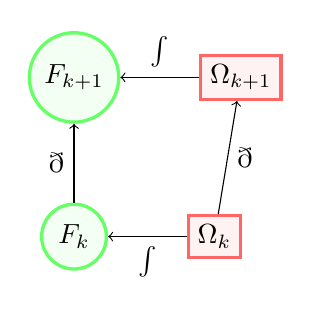
\begin{tikzpicture}
[roundnode/.style={circle, draw=green!60, fill=green!5, very thick, minimum size=7mm},
squarednode/.style={rectangle, draw=red!60, fill=red!5, very thick, minimum size=5mm},
]
\node[roundnode]	(f2) {$F_{k+1}$};
\node[roundnode]	(f1) [below=of f2]{$F_k$};
\node[squarednode]	(w2) [right=of f2] {$\Omega_{k+1}$};
\node[squarednode]	(w1) [right=of f1] {$\Omega_k$};

\draw[<-] (f2) -- (w2) node[midway, above] {$\int$};
\draw[<-] (f2) -- (f1) node[midway, left] {$\eth$};
\draw[<-] (f1) -- (w1) node[midway, below] {$\int$};
\draw[<-] (w2) -- (w1) node[midway, right] {$\eth$};
\end{tikzpicture}





\begin{defn}
	\textbf{Stokes' Theorem}: For (k-1)-form $\omega$ and k-surface $\sigma$, $\int_{\partial \sigma}\omega = \int_{\sigma}\eth\omega$. \textbf{NOTE: We kinda already gave this definition in the exterior derivative deifnition. It's kinda funny. We can handle this two ways: define the exterior derivative as being an operation that does the thing, and have stoke's theorem be waht the exterior derivative does. }
\end{defn}

In many treatments of Electromagnetism (for example, "Classical Electromagnetic Radiation" by Heald and Marion), Stokes' Theorem is given in terms of the curl as \begin{gather}\int_S \nabla \times \vec{A} \cdot d\vec{S} = \oint_{\Gamma} \vec{A} \cdot d\vec{l}\end{gather} (\textbf{Figure out how to categorize these terms}). This allows us to take a brief digression to see how the tools we have defined look in the more familiar 3D cases. 

\textbf{Introduce this wedge-product formulation of the k-form before this}

In general, we have that for $\omega_k \in \Omega_k$, \begin{gather}\omega_k = \omega_{ab...c}e^a\wedge e^b \wedge ... \wedge e^c,\end{gather} and \begin{gather} \eth \omega_k = \partial_a\omega_{bc...d}e^a\wedge e^b\wedge e^c\wedge ... \wedge e^d.\end{gather} So, suppose we have $f \in \Omega_0$, $v \in \Omega_1$, and $B \in \Omega_2$, and we apply the exterior derivative to each of them. We have that \begin{gather}\eth f = \partial_a f e^a,\end{gather} \begin{gather}\eth v = \partial_a v_b e^a \wedge e^b,\end{gather} and \begin{gather}\eth B = \partial_a B_{bc} e^a\wedge e^b \wedge e^c.\end{gather} 

By looking closer at these expressions, we see familiar tools from vector calculus arise. $\partial_a f e^a$ is a 1-form consisting of the sum of derivatives in each of the basis directions. In the 3D case, we have that \begin{gather}\partial_a f e^a = \frac{\partial f}{\partial x^1} e^1 + \frac{\partial f}{\partial x^2} e^2 + \frac{\partial f}{\partial x^3} e^3.\end{gather} This is simply the gradient of a scalar functional. So, we have that in $\mathbb{R}^3$, \begin{gather}\partial_a f e^a = \nabla f.\end{gather} Similarly, we see that in 3D, $\eth v$ will give us a 2-form from a 1-form, composed of the sum of derivatives in the directions perpendicular to the original 1-form. That is, in $\mathbb{R}^3$, \begin{gather}\eth v = (\frac{\partial v_2}{\partial x^3} - \frac{\partial v_3}{\partial x^2})e^2\wedge e^3 - (\frac{\partial v_1}{\partial x^3} - \frac{\partial v_3}{\partial x^1})e^1 \wedge e^3 + (\frac{\partial v_1}{\partial x^2} - \frac{\partial v_2}{\partial x^1})e^1 \wedge e^2.\end{gather} Finally, \begin{gather} \eth B = (\frac{\partial B_1}{\partial x^1} + \frac{\partial B_2}{\partial x^2} + \frac{\partial B_3}{\partial x^3})e^1\wedge e^2 \wedge e^3.\end{gather} We see here that $\eth v$ doesn't \emph{quite} give us $\nabla \times v$, and $\eth B$ doesn't \emph{quite} give us $\nabla \cdot B$. This discrepancy demonstrates the difference between the wedge product and the cross product. Had we done $\nabla \times v$, the first term would have been $(\frac{\partial v_2}{\partial x^3} - \frac{\partial v_3}{\partial x^2})e^1$. That is, in the direction perpendicular to $e^2\wedge e^3$. This is similarly true for the components in $e^1\wedge e^3$ and $e^1 \wedge e^2$. Furthermore, $\nabla \cdot B$ returns a scalar (i.e., no direction), while $\eth B$ returns a single value in the $e^1 \wedge e^2 \wedge e^3$ "direction." This discrepancy is resolved by the introduction of the Hodge Dual Operator $*$, such that $*\eth v = \nabla \times v$ and $*\eth B = \nabla \cdot B$, but this is beyond us at the moment. What does hold immediately true is a generalization of the expression \begin{gather} \nabla \times \nabla V = 0\end{gather} for any scalar function $V$. For any form $\omega_k \in \Omega_k$, we have that \begin{gather} \eth\eth\omega_k = 0.\end{gather}

With these new, more general geometric expressions for gradient, curl, and divergence, their physical interpretations become immediately clear, simply from the notation. If we extend the flux example, we see that the gradient of a 0-form is simply the lengthwise flow in each possible dimension (three, in 3D), the curl of a 1-form is the planewise flow in each plane (still 3, in 3D), and the divergence of a 2-form is the flow outwards from a point per unit volume. 



\section{Closed and Exact Forms, and Potentials}





\section{Electricity and Magnetism}

\textbf{In order to do this, need a hodge dual, so need perpendicular, so need a metric. Otherwise can only have curl of E equals derivative of B in t. }

- We have work, this relates to force, and the electric field (magnetic field does no work)

- We can relate the electric force to a potential using the boundary functional (i.e. $f_e = -\eth\phi$)

- Define the field strength tensor


\textbf{NOTE: In fluid dynamics for divergenceless fluid, there's something called stream functions}

\textbf{Bohm: If the form is closed, then the exterior derivative is always zero, thus all the integrals on closed surface that can be shrunk to a point will be zero. So, taking a convex region, we can create a potential there. z.B. assume we have a line}

\textbf{If it happens that the number for all closed surfaces (small enough up to a certain point) are always zero, then the form/functional is cosed. If it's zero on all the closed k-surfaces we give it, then its exact. The difference is that both admit potentials, but the closed form is only going to admit a potential in a convex region small enough where al the closed surfaces are zero. The exact will admit a potential globally (an n-1 form/functional that if given the exterior derivative gives the original thing)}

\textbf{Closed if for some set, all closed surfaces give zero for the functional. Exact if that open region corresponds to the whole space. Closed implies exact, but not the other way around}







\chapter{Geometry and (States, Tensors, Forms)???}

\emph{Two types of geometry: symplectic which only has 2D areas, and riemannian which has length and angles}


\section{Symplectic geometry and state spaces}
We want to be able to represent our state configurations. Symplectic geometry arises when trying to describe their areas

\subsection{Symplectic form and areas}



\subsection{Metric tensor}
A more generalized inner product: feed in two vectors, and the outcome is a scalar representing the lengths of the vectors and the angle between them. 

\begin{defn}
	A \textbf{metric tensor g} is a function that takes two vectors and returns a real scalar. 
\end{defn}


\section{Riemannian geometry}
In order to give a mathematically rigorous definition of lengths of vectors and the angle between them, we use an inner product. Vector spaces with an inner product are Riemannian.

\begin{defn}
	Given two vectors $X^a,Y^a \in V$ and a metric tensor $g_{ab}$, the \textbf{inner product} $<X^a,Y^a> : V \times V \to \mathbb{R}$ is defined as $<X^a,Y^a> = g_{ab}X^aY^b$. 
\end{defn}

\begin{coro}
	The magnitude of $<u,v>$ is $|u||v|cos(\theta)$, where $\theta$ is the angle between u and v. 
\end{coro}

\begin{defn}
	If a vector space V contains an inner product, then V is \textbf{Riemannian}.
	\end{defn}



\subsection{Orthogonal basis}

\begin{defn}
	For contravariant vectors $X^a$ and $Y^a$, the two vectors are \textbf{orthogonal} if $<X^a,Y^b> = 0$. 
\end{defn}







\end{document}